\documentclass{standalone}
\usepackage{tikz}
\begin{document}
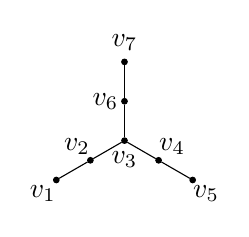
\begin{tikzpicture}[every node/.style={draw, circle, fill=black, minimum size=2pt, inner sep=0pt}]
\node[fill=black, label=below left :{$v_{1}$}] (G1N4) at (210:1) {};
\node[fill=black, label=above left:{$v_{2}$}] (G1N1) at (210:0.5) {};
\node[fill=black, label=below:{$v_{3}$}] (G1N0) at (0:0) {};
\node[fill=black, label=above right:{$v_{4}$}] (G1N2) at (330:0.5) {};
\node[fill=black, label=below right:{$v_{5}$}] (G1N5) at (330:1) {};
\node[fill=black, label=left:{$v_{6}$}] (G1N3) at (90:0.5) {};
\node[fill=black, label=above:{$v_{7}$}] (G1N6) at (90:1) {};
\draw (G1N0) -- (G1N1);
\draw (G1N0) -- (G1N2);
\draw (G1N0) -- (G1N3);
\draw (G1N1) -- (G1N4);
\draw (G1N2) -- (G1N5);
\draw (G1N3) -- (G1N6);
\end{tikzpicture}
\end{document}
